\subsection{Base y principio de diseño}
La aplicación fundamental de las antenas es la transmisión y recepción de información empleando, para ello, radiación electromagnética. También, como es el caso de la tecnología RFID utilizada en el proyecto, una de las antenas (PICC) toma energía del flujo magnético generado por la otra (PCD), energizandose.

Para lograr el cumplimiento de la norma sobre RFID ISO 14443 Tipo A logrando, así, la comunicación entre el PCD y el PICC se deben tener en cuenta las características de la comunicación:

\begin{itemize}
\item Frecuencia de portadora.
\item Frecuencia de subportadoras.
\item Modulación ASK 100\% desde el PCD al PICC.
\item Modulación de carga desde el PICC al PCD.
\end{itemize}

Además de las características que debe tener una antena ante la transmisión de información, se debe tener en cuenta la distancia entre antenas entre las cuales es alcanzable el funcionamiento de la comunicación, para este factor de los sistemas RFID, se debe tener en cuenta:

\begin{itemize}
\item Tamaño de antena PCD (y PICC)
\item Emparejamiento de la antena
\item Factor de calidad de la antena y circuito de adaptación
\item Potencia de la PCD
\item Influencias medioambientales
\end{itemize}

\subsection{Funcionamiento del sistema}

La corriente en la antena del PCD genera un flujo magnético Φ. Partes de este flujo Φ fluye a través de la bobina de la tarjeta e induce un voltaje. Esta tensión se rectifica y el IC de la tarjeta se activa cuando se alcanza la tensión de funcionamiento.
El voltaje inducido variará dentro de la distancia entre la antena PCD y el PICC. Debido a esa variación, la distancia de operación alcanzable está limitada por la potencia transferida.

Basado en el principio del transformador (Figura \ref{fig:trafo}) y en la leyes de Faraday para electromagnetismo, puede calcularse la densidad media del flujo y así la tensión inducida en dependencia del ángulo de operación, el radio y espiras de la antena del PICC. Basándose, además, en el límite de la intensidad de campo mínima requerida como se especifica en ISO14443-2 (Sección \ref{sec:iso}).

\begin{figure}[H]
\centering
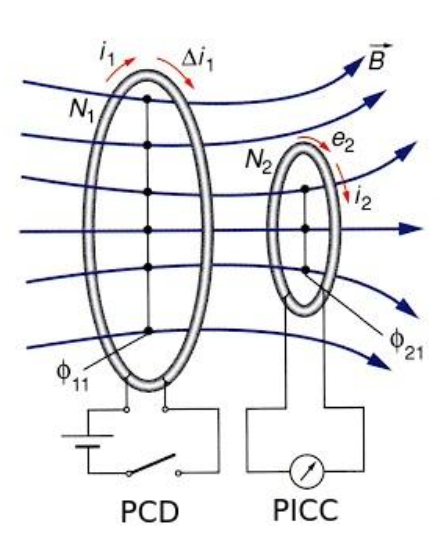
\includegraphics[scale=0.6]{antena/antena_trafo.png}
\caption{Densidad de flujo magnético generada por el PCD e inducida en la antena del PICC.}
\label{fig:trafo}
\end{figure}

La Figura \ref{fig:acople} muestra el factor de acoplamiento K frente al diámetro de antena D en base a la distancia de operación requerida de 10 cm.
Aunque la curva es muy plana en su parte superior, se puede ver que un diámetro de antena menos de 15 cm muestra una disminución significativa del factor de acoplamiento (y rendimiento). El factor de acoplamiento y el rendimiento disminuye drásticamente cuando el diámetro de la antena es inferior a 12 cm.

\begin{figure}[H]
\centering
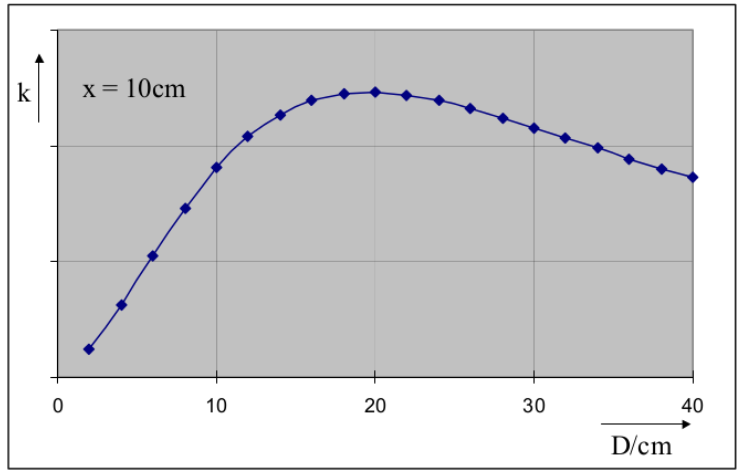
\includegraphics[scale=0.5]{antena/antena_acople.png}
\caption{Factor de acoplamiento vs Diámetro de la antena.}
\label{fig:acople}
\end{figure}

El inductor del PICC ($L_{PICC}$) está acoplado a la antena del transponder ($L_{PCD}$), existiendo así una inductancia mutua M entre ellos (Figura C). Esta inductancia mutua puede definirse en función de las inductancias de las antenas y el coeficiente de acoplamiento (k) como:
\begin{equation}
M = k \sqrt{L_{PCD}L_{PICC}}
\end{equation}

\begin{figure}[H]
\centering
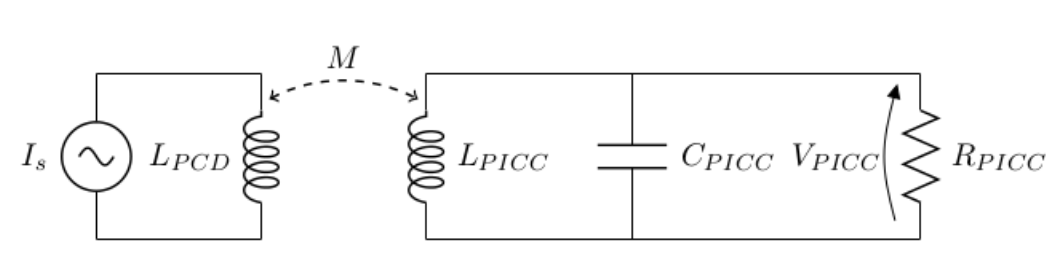
\includegraphics[scale=0.5]{antena/antena_m.png}
\caption{Modelo simplificado del acoplamiento inductivo entre el PCD y el PICC.}
\label{fig:acoplem}
\end{figure}

Cabe destacar que la relación mostrada anteriormente entre el tamaño de la antena y la distancia de operación es independiente del número de espiras (y la inductancia) de la antena PCD.
El coeficiente de acoplamiento es un factor limitante no sólo para la energía que se transporta al PICC, sino también para la respuesta del PICC que debe ser recibida por el PCD.


\subsection{Modelo de simulación}

En la nota de aplicación de Zheng Zhu \cite{shunt1}, se detalla el modelo de simulación para una antena HF RFID. El modelo se muestra en la figura \ref{fig:ant_model} y los valores de los componentes en la tabla \ref{table:sim_values}.

\begin{figure}[H]
\centering
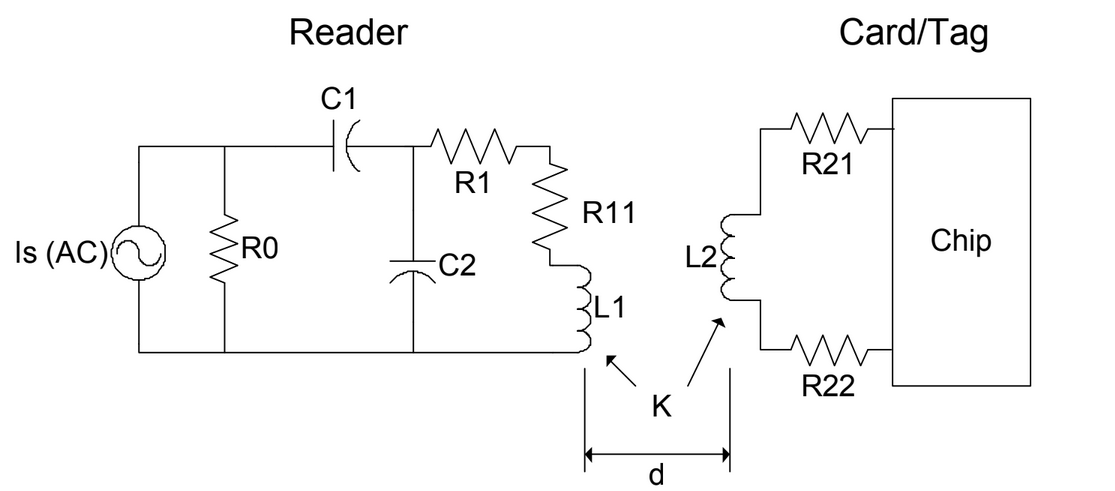
\includegraphics[width=0.9\linewidth]{antena/antena_model.png}
\caption{Modelo de simulación de una antena en HF}
\label{fig:ant_model}
\end{figure}

\begin{table}[h]
\centering
\caption{Valores de los componentes para el modelo de simulación}
\label{table:sim_values}
\begin{tabular}{c|c|c}
Componentes & Explicación                           & Valores típicos                      \\ \hline
Is          & Fuente de corriente ideal             & 162 mA efectivos (AC) para 13.56 MHz \\
R0          & Resistencia de la fuente de corriente & 50                                   \\
C1          & PCD circuito de matching              & 47 pF                                \\
C2          & PCD circuito de matching              & 184 pF                               \\
R1          & PCD circuito de matching              & 2                                    \\
R11         & Resistencia de la antena PCD          & 0.2                                  \\
L1          & Inductancia de la antena PCD          & 0.6 uH                               \\
L2          & Inductancia de la antena PICC         & 4.08 uH                              \\
R21, R22    & Resistencia de la antena PICC         & 1.32                                 \\
K           & Factor de acople                      & 0.008 (15 cm), 0.12 (0 cm)          
\end{tabular}
\end{table}

\clearpage

